\section{Evaluation}
\label{sec:evaluation}

We answer five research questions using the task-aligned v1 artifacts. As defined in Section~\ref{sec:methodology}, unresolved designators are excluded and exact cross-class bytecode conflicts are quarantined. G-DET, G-MUT, G-VOL, and G-ADV retain their distinct splits, thresholds, and transformation conditions; values across these groups are not treated as one before/after experiment.

\subsection{RQ1: Family-Grouped Detection}

\emph{How accurately does AuthGuard separate artifact-derived positives from rule-silent weak negatives when related families are held out?} Table~\ref{tab:gdet-performance} reports G-DET on 727 positives and 1,553 \texttt{benign\_cleared} observations. AuthGuard has the highest AUPRC among the evaluated non-tautological methods, $0.881\pm0.028$, followed by opcode-histogram XGBoost at $0.784\pm0.081$. Its mean AUROC is 0.943, with precision 0.869 and recall 0.576 at fitting-prediction thresholds.

\begin{table}[t]
  \centering
  \caption{G-DET on 727 artifact-derived positives and 1,553 weak negatives. Values are five preserved family-fold means; AUPRC reports population SD, and thresholded metrics use fitting-prediction maximum-$F_1$ thresholds.}
  \label{tab:gdet-performance}
  \scriptsize
  \setlength{\tabcolsep}{2.0pt}
  \begin{tabular}{@{}lccccc@{}}
    \toprule
    Method & \shortstack{AUPRC\\$\pm$ SD} & AUROC & Prec. & Rec. & $F_1$ \\
    \midrule
    Sens.-name approx. & $.344\pm.094$ & .520 & .884 & .043 & .079 \\
    Ext.-call over-approx. & $.328\pm.078$ & .518 & .328 & 1.000 & .489 \\
    Exact-hash blocklist & $.321\pm.077$ & .500 & .000 & .000 & .000 \\
    Selector-LR & $.515\pm.066$ & .666 & .449 & .618 & .512 \\
    Opcode-histogram RF & $.744\pm.085$ & .878 & .842 & .297 & .426 \\
    Opcode-histogram XGB & $.784\pm.081$ & .883 & .798 & .544 & .626 \\
    AuthGuard & $\mathbf{.881\pm.028}$ & \textbf{.943} & .869 & .576 & .673 \\
    \bottomrule
  \end{tabular}
  \vspace{1pt}

  \parbox{\columnwidth}{\scriptsize Sens.: sensitive; Ext.: external; XGB: XGBoost; Prec./Rec.: precision/recall.}
\end{table}


The external-call structural over-approximation reaches 1.000 recall but only 0.328 AUPRC and 0.328 precision, indicating that merely observing a call-family opcode does not discriminate this population. Conversely, the exact-hash blocklist has zero held-out-family recall. The sensitive-name rule approximation is precise when it fires (0.884) but reaches only 0.043 recall. These local rules do not reproduce the full USENIX Gigahorse/Datalog pipeline, which we did not run, and Table~\ref{tab:gdet-performance} does not compare AuthGuard with that system. The labels also bound the inference: positives derive from its artifact and \texttt{benign\_cleared} is weak-negative rather than verified benign ground truth. Separate independent sourcing yielded only one confirmed novel positive, which is insufficient for quantitative external validation.

\subsection{RQ2: Random-Split Optimism}

\emph{How optimistic is random evaluation when related bytecode can cross splits?} Figure~\ref{fig:random-family} pairs family-grouped and seeded-random G-DET AUPRC. AuthGuard rises from 0.881 to 0.975, an absolute gap of 0.094. Larger gaps occur for the exact-hash blocklist (0.321 to 0.551), opcode-histogram RF (0.744 to 0.969), and opcode-histogram XGBoost (0.784 to 0.965); selector-LR changes from 0.515 to 0.559.

\begin{figure}[t]
  \centering
  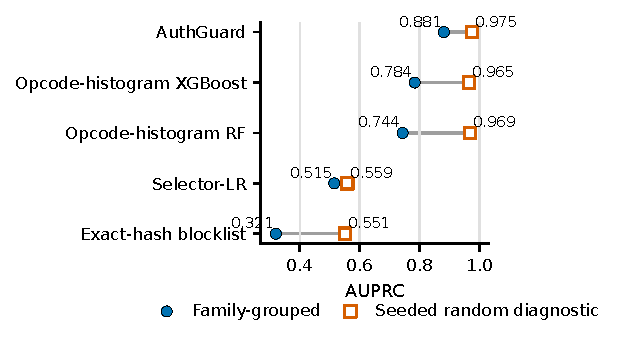
\includegraphics[width=\columnwidth]{figures/random_vs_family.pdf}
  \caption{G-DET five-fold mean AUPRC for task-aligned positives versus weak negatives. The seeded random split is a diagnostic on this corpus; family-grouped testing controls related-bytecode leakage and provides a more demanding generalization estimate.}
  \label{fig:random-family}
\end{figure}

The blocklist gap directly demonstrates that exact duplicates can cross the random split, while the learned-model gaps are consistent with dependence beyond exact identity. The family construction is a bytecode-similarity grouping, not attacker attribution. It controls an identified dependence source but does not remove every form of memorization or imply that every random-split study is invalid.

\subsection{RQ3: Mutation and Flooding Stress Tests}

\emph{How do the evaluated methods respond to checker-defined bytecode transformations?} G-MUT fits learned models on clean M0 families and transforms only held-out positives. Table~\ref{tab:gmut-robustness} shows retained recall. The sensitive-name approximation remains at 0.043 through M2 and falls to zero when M3 rewrites matching selector immediates. The external-call over-approximation remains at 1.000 because its broad all-positive behavior is unaffected; its poor G-DET discrimination prevents interpreting this as useful robustness. The exact-hash blocklist remains at zero. AuthGuard changes from 0.576 on M0 to 0.530 on M3, while selector-LR and opcode-histogram XGBoost reach 0.613 and 0.463 at M3.

\begin{table}[t]
  \centering
  \caption{G-MUT five-fold mean retained recall on held-out positive families under cumulative M0--M3 transformations. All 727 positives passed the opcode-token checker at M1--M3; this is not an execution-equivalence test.}
  \label{tab:gmut-robustness}
  \scriptsize
  \setlength{\tabcolsep}{3.2pt}
  \begin{tabular}{@{}lcccc@{}}
    \toprule
    Method & M0 & M1 & M2 & M3 \\
    \midrule
    Sens.-name approx. & .043 & .043 & .043 & .000 \\
    Ext.-call over-approx. & 1.000 & 1.000 & 1.000 & 1.000 \\
    Exact-hash blocklist & .000 & .000 & .000 & .000 \\
    Selector-LR & .618 & .619 & .614 & .613 \\
    Opcode-histogram XGB & .544 & .603 & .463 & .463 \\
    AuthGuard & .576 & .608 & .530 & .530 \\
    \bottomrule
  \end{tabular}
  \vspace{1pt}

  \parbox{\columnwidth}{\scriptsize Sens.: sensitive; Ext.: external; XGB: XGBoost.}
\end{table}


All 727 retained positives passed the repository's pre-metadata opcode-token checker at M1, M2, and M3. This supports only the stated syntactic invariant; it does not prove EVM execution or behavioral equivalence.

Figure~\ref{fig:mutation-flooding}(b) separately reports G-VOL. At its compound metadata/address/selector starting condition, AuthGuard and opcode-histogram XGBoost retain 0.608 and 0.603 recall. With post-STOP flooding intended to model padding at +200\%, they fall to 0.130 and 0.279, respectively. The sensitive-name approximation remains zero and the external-call over-approximation remains one throughout. Thus heavy compound flooding is a demonstrated residual weakness. G-VOL is not the pure-M0 F200 condition used by G-ADV, and no augmentation-recovery claim is made for it.

\begin{figure*}[t]
  \centering
  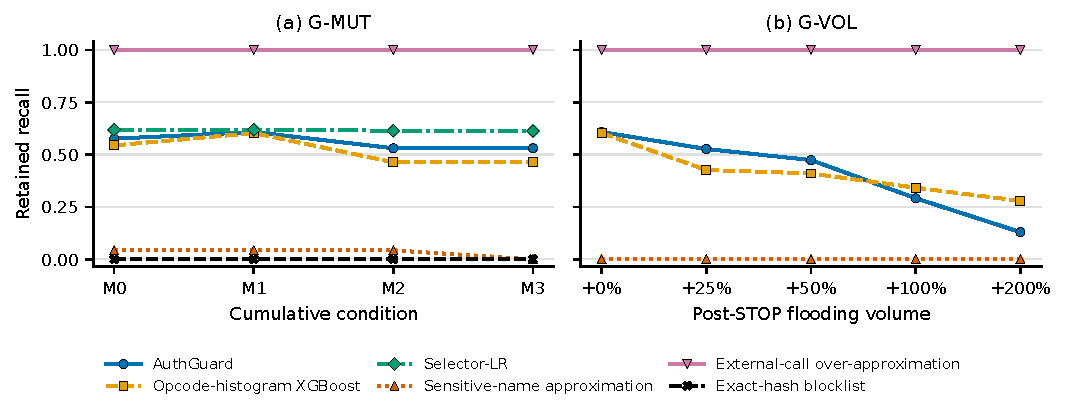
\includegraphics[width=\textwidth]{figures/mutation_and_flooding.pdf}
  \caption{Five-fold mean retained recall on held-out positive families under (a) G-MUT cumulative M0--M3 transformations and (b) G-VOL compound metadata/address/selector transformation with post-STOP flooding intended to model dead-code padding. G-MUT/G-VOL use clean-model thresholds. G-VOL is not the G-ADV pure-M0 F200 experiment.}
  \label{fig:mutation-flooding}
\end{figure*}

\subsection{RQ4: Adversarial Augmentation}

\emph{Does source-balanced, family-disjoint augmentation improve held-out-condition performance?} Table~\ref{tab:gadv-results} reports G-ADV. On clean M0, AuthGuard-M0 versus AuthGuard-aug yields AUPRC/recall/FPR of $0.819/0.759/0.134$ versus $0.863/0.807/0.108$. On held-out M3, the corresponding values are $0.768/0.767/0.181$ and $0.825/0.796/0.120$. Figure~\ref{fig:gadv-heldout} visualizes these fold means without treating fold dispersion as paired uncertainty.

\begin{table*}[t]
  \centering
  \caption{G-ADV five-fold means on clean M0 and held-out M3 and pure-M0 F200. AUPRC is threshold-free; precision, recall, and benign FPR use thresholds selected on separate clean-M0 validation families. XGB denotes XGBoost; bold marks the best value per condition and metric.}
  \label{tab:gadv-results}
  \small
  \setlength{\tabcolsep}{6pt}
  \begin{tabular}{@{}llcccc@{}}
    \toprule
    Condition & Model & AUPRC & Precision & Recall & FPR \\
    \midrule
    Clean M0 & Opcode-histogram XGB & .757 & .677 & .661 & .161 \\
             & Opcode-histogram XGB-aug & .752 & .610 & .779 & .284 \\
             & AuthGuard-M0 & .819 & .720 & .759 & .134 \\
             & AuthGuard-aug & \textbf{.863} & \textbf{.763} & \textbf{.807} & \textbf{.108} \\
    \midrule
    Held-out M3 & Opcode-histogram XGB & .695 & .640 & .675 & .201 \\
                & Opcode-histogram XGB-aug & .723 & .600 & \textbf{.807} & .304 \\
                & AuthGuard-M0 & .768 & .663 & .767 & .181 \\
                & AuthGuard-aug & \textbf{.825} & \textbf{.743} & .796 & \textbf{.120} \\
    \midrule
    Held-out pure-M0 F200 & Opcode-histogram XGB & .529 & .489 & .601 & .347 \\
                          & Opcode-histogram XGB-aug & .696 & .538 & \textbf{.756} & .386 \\
                          & AuthGuard-M0 & .561 & .512 & .484 & .217 \\
                          & AuthGuard-aug & \textbf{.758} & \textbf{.654} & .727 & \textbf{.174} \\
    \bottomrule
  \end{tabular}
\end{table*}


\begin{figure*}[t]
  \centering
  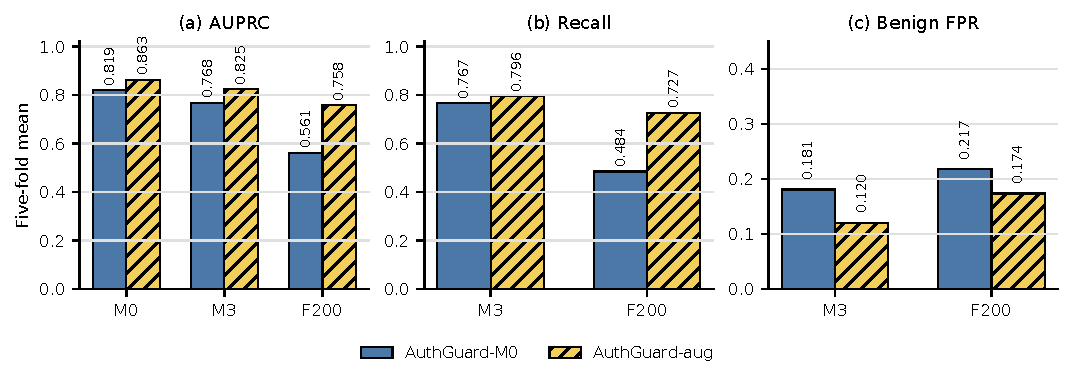
\includegraphics[width=\textwidth]{figures/advtrain_heldout.pdf}
  \caption{G-ADV five-fold means for AuthGuard-M0 and AuthGuard-aug. Panel (a) reports threshold-free AUPRC on clean M0 and held-out M3 and pure-M0 F200; panels (b)--(c) report recall and benign FPR at clean-validation thresholds on held-out conditions. Family-clustered paired intervals are reported separately in the text.}
  \label{fig:gadv-heldout}
\end{figure*}

On held-out pure-M0 F200, fold-mean AUPRC/recall/FPR moves from $0.561/0.484/0.217$ to $0.758/0.727/0.174$. This is an aggregate discrimination improvement under the tested severity, but the remaining 0.174 FPR is material. Moreover, opcode-histogram XGBoost-aug reaches higher recall (0.756) than AuthGuard-aug (0.727), whereas AuthGuard-aug has higher AUPRC (0.758 versus 0.696) and lower FPR (0.174 versus 0.386). AuthGuard therefore offers the better ranking/false-positive trade-off here, not dominance on every metric.

For paired inference, 10,000 replicates resample all 819 frozen test families, retaining their 2,280 observations and model pairing. At F200, pooled recall changes from 0.448 to 0.702; the augmented-minus-M0 difference is $+0.253$ (95\% CI $[0.144,0.379]$). Pooled FPR changes from 0.228 to 0.179, a $-0.049$ difference (95\% CI $[-0.086,-0.014]$), and the AUPRC difference is $+0.248$ (95\% CI $[0.177,0.322]$). These family-clustered intervals exclude zero. Clean and M3 recall differences do not: $+0.044$ $[-0.045,0.133]$ and $+0.023$ $[-0.040,0.080]$, respectively. Their FPR differences are supported: clean $-0.024$ $[-0.048,-0.001]$ and M3 $-0.059$ $[-0.083,-0.037]$. Thus clean and M3 recall increases are not statistically established. The results support improvement under the tested held-out transformations, not arbitrary-transformation robustness, and do not resolve compound G-VOL F200.

\subsection{RQ5: Local Processing Cost}

\emph{What is the cost of the implemented local scoring path?} On an Apple M1, preloaded-bytecode normalization, feature extraction, and prediction averaged 3.411\,ms per contract over 3,000 single-contract calls; p95 was 9.514\,ms. Ten timed 300-contract batches averaged 3.197\,ms per contract. This scorer-core measurement excludes model loading, authorization parsing, RPC/network retrieval, caching, wallet integration, and warning rendering. It is therefore not end-to-end wallet latency and does not by itself validate a deployed interactive system.
